\documentclass[letterpaper,10pt]{article}

\usepackage[english]{babel}
\usepackage[utf8]{inputenc}
\usepackage{amsmath}
\usepackage{graphicx}
\usepackage[colorinlistoftodos]{todonotes}
\usepackage[top=1in, bottom=0.5in, left=1in, right=1in]{geometry}
\usepackage[small]{titlesec}

\newcommand{\bes}{\begin{equation*}}
\newcommand{\ben}[1]{\begin{equation}\label{#1}}
\newcommand{\ees}{\end{equation*}}
\newcommand{\be}{\begin{equation}}
\newcommand{\ee}{\end{equation}}

\begin{document}

\begin{flushright}
{\Large Josh Bevan - HW 4 Q2 - CS556}
\end{flushright}
\vskip -0.1in
\hrule
\vskip 0.3in

\hskip -.3in{\large \textit{Implement ILU(0) for CSR matrices with the following prototype...}}

\section*{Now test your ILU(0) by using it to create a preconditioner for GMRES. For each case, consider both how well ILU(0) preconditions GMRES in terms of number of iterations and the practical effectiveness of the preconditioner for solving the problem. Consider any $b$ you choose and two different matrices:}
The built-in gmres() implementation in scipy.sparse.linalg was used. The solution vector $b$ was chosen to be random, but the same random vector was used when comparing all 4 cases. A linear operator via a lambda function was used in lieu of directly inverting the preconditioning matrix (per the documentation recommendations of scipy.sparse.linalg.gmres()). Also, a callback function was used to retain the number of iterations and the residual convergence history of each gmres() solve for later inspection. The tolerance was set to be near single precision, 1e-8; the restart frequency was left at default, 20. The size of the A matrices examined varied between 36x36 up to 4500x4500. The density chosen for the random matrix cases was 0.1.

\subsection*{The 2D Poisson stencil matrix}
The 2D Poisson stencil case was largely consistent across the range of mesh sizes examined. The example figures in Figure 1 presented are typical of the results obtained; both the PC and non-PC versions reliably converged to the desired tolerance for the range of A matrices examined. Also similar across all runs was that the preconditioned version converged to the desired tolerance in fewer iterations. For small matrices it converged in about half the iterations. As the size of the A matrix increased there was weak scaling observed in the reduction of iterations necessary of the PC version compared to the same non-PC version. Figure 2 plots the this scaling for the range of sizes examined. Based on the observed behavior it seems ILU(0) is a satisfactory preconditioned for this type of matrix.

\begin{figure}[!htb]
\hskip -0.6in
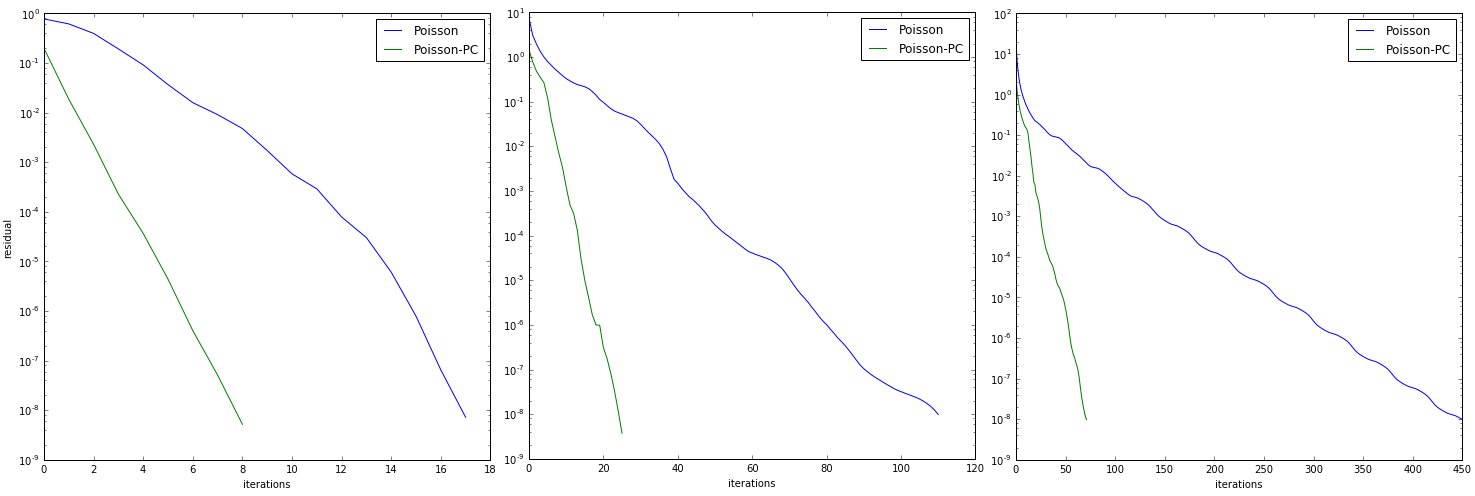
\includegraphics[width=1.2\textwidth]{PoissonABC.PNG}
\caption{Convergence history of the residuals for the non-PC and PC versions of the 2D Poisson stencil case. Left to right: 36x36, 400x400, 2500x2500 $A$ matrix.}
\end{figure}

\begin{figure}[!htb]
\centering
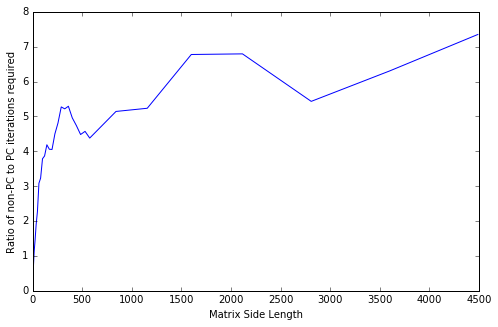
\includegraphics[width=0.7\textwidth]{PoissonRat.PNG}
\caption{Increasing effectiveness of preconditioning at reducing number of iterations required (compared to non-PC) as Poisson matrix size increases.}
\end{figure}

\subsection*{The matrix resulting from $A=I+SA=I+S$ where $I$ is the identity matrix and $S$ is the random sparse matrix generated by sprand}
The situation for the use of the ILU(0) preconditioner for the random matrix is different compared to the Poisson case. Before even considering the effect of the preconditioner, it is notable that the number of iterations required to converge to the same tolerance for the same size problem as the Poisson case is much higher. This is perhaps not surprising given that we can't say nearly as much about the conditioning of the random A matrix.

 Figure 3 plots the 3 types of phenomena observed for the preconditioner. For cases where GMRES was able to converge to the desired tolerance, the preconditioned version converged in far fewer iterations. There were other cases where the preconditioned GMRES converged while the non-PC version did not. Finally, there were other cases where neither converged to the desired tolerance; in this case the preconditioned version was actually typically worse.
 
 An important consideration in the applicability of the ILU(0) preconditioner is how well it represents the true LU decomposition. Ideally it would be quite close to the true LU decomposition, in which case it will be quite effective. In the Poisson test case the banded nature of the matrix means there is comparatively less fill-in compared to the random matrix case where there is much more fill-in for the true LU decomposition. Commensurately, the ILU(0) preconditioner for the random matrix case will be farther from the true LU decomposition and therefore more dependent on the sparsity pattern of the random matrix. In this sense the choice of the ILU(0) preconditioner will lead to inconsistent performance of GMRES.
\begin{figure}[!htb]
\hskip -0.6in
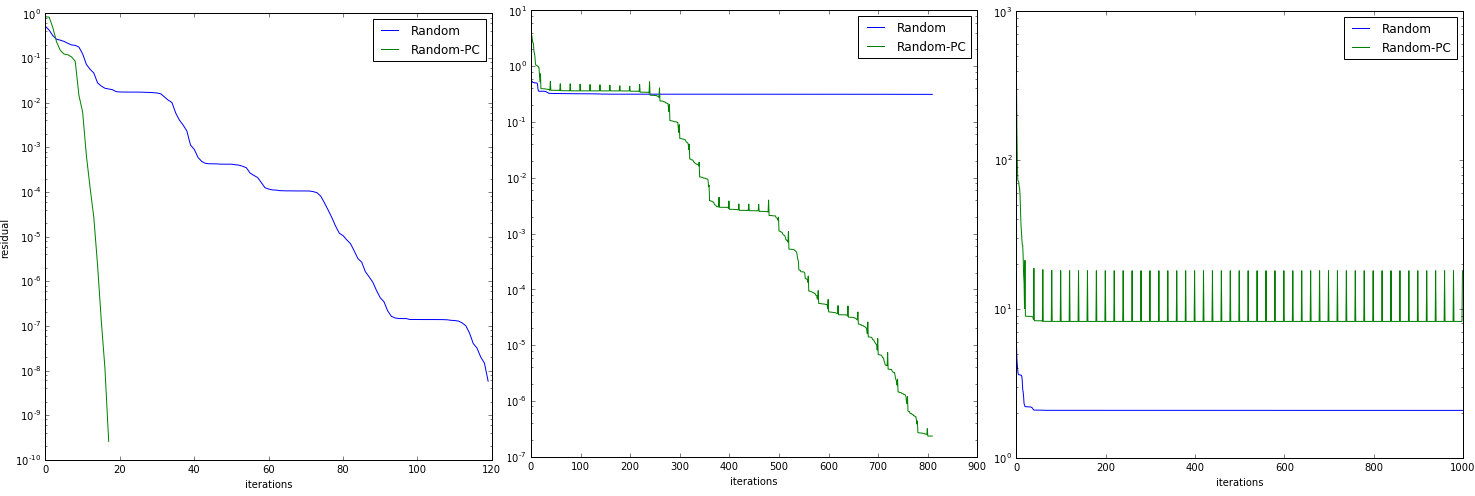
\includegraphics[width=1.2\textwidth]{RandomABC.PNG}
\caption{Convergence history of the residuals for the non-PC and PC versions of the random $R+I$ case. Left to right: 36x36, 81x81, and 100x100 $A$ matrix}
\end{figure}

\end{document}